% ---------------------------------------------------------------------
\chapter{Introduction}
% ---------------------------------------------------------------------
\section{Task}
According to the task, there are two functions, namely the synthesis of object point cloud information and object recognition and tracking. These functions will be based on the ROS operating system using the C++ programming language.
In the first task, because the image collected by one camera is incomplete, it is necessary to use two cameras to collect information together, and then synthesize complete object information. First, you need to use two realsence D435i cameras to collect the point cloud information of the object, and then use the rotation matrix to unify the coordinate systerm of the obtained information, then perform the point cloud information fusion, and finally filter to obtain the final composite image.
The second task is tracking and identifying objects.
\section{Motivation}
Computer engineering students need not only knowledge of algorithms and computers, but also programming skills in order to find good and suitable jobs in the future.
Through small seminars, we should use the object-oriented programming language C++ to complete the task on the ROS system.
At the same time, project development experience can also be obtained.
In recent years, the Python programming language has been more popular on the market. However, some programming languages such as C++ with pointers reflect some of the development principles of computers in software and hardware. Therefore, with the help of C++ knowledge, we can be faster and easier to master other programming languages, such as Java and Python.\\
\begin{figure}[htp]
	\centering % 图片居中
	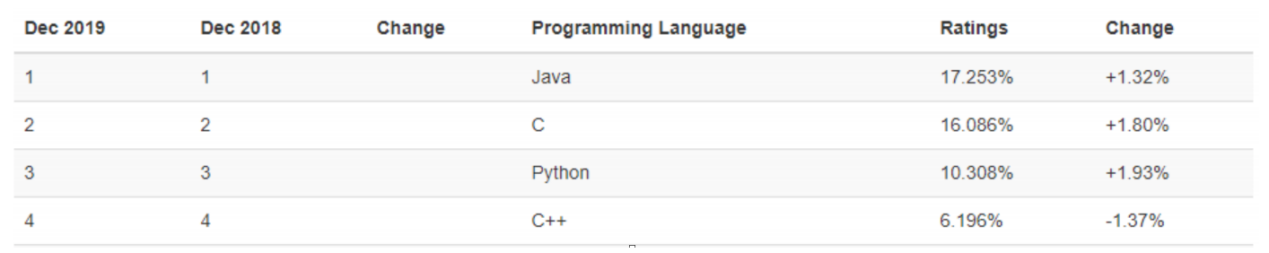
\includegraphics[width = 15.3cm]{figures/Motivation}
	\caption{Ranking list of programming languages in Tobi}
	\label{fig:figure1label}
\end{figure}

In addition, the required functions must be implemented in Linux. The code has been integrated into the Linux command line. So you can also understand the operating system, which covers a wide range of fields, even in short-term papers.



	
